\documentclass{beamer}
\usepackage[utf8]{inputenc}
\usepackage[spanish]{babel}
\usepackage{hyperref}
\usepackage{graphicx}
\usepackage{wrapfig}
\usepackage[square,numbers]{natbib}
%\bibliographystyle{unsrtnat}

\hypersetup{
    colorlinks=true,
    linkcolor=blue,
    filecolor=magenta,      
    urlcolor=cyan,
}

\usetheme{Madrid}
\usecolortheme{default}

\title[Procesamiento de Imágenes] 
{Fast and Efficient Method for
Fire Detection Using Image Processing}
\author[Joaquín Laks, Bianca Bramati] 
{Joaquín Laks, Bianca Bramati}
\institute[] 
{
  Procesamiento de Imágenes\\
  2° Cuatrimestre 2024 \\
}
\date{}

\begin{document}
\frame{\titlepage}
\section{Nombre de la sección}
\begin{frame}
\frametitle{Nombre de la diapositiva}
El paper \textit{Fast and Efficient Method for Fire Detection Using Image Processing}$^1$ presenta un método para \textbf{detectar fuego en videos}, en dos pasos:
\begin{enumerate}
    \item Segmentar el fuego en cada frame de forma estática, en base a un modelo de color.
    \item Detectar movimiento de píxeles entre frames contiguos. 
\end{enumerate} 
\end{frame}

\section{Objetivos}
\begin{frame}
\frametitle{Objetivos}
\begin{enumerate}
    \item Replicar los resultados obtenidos en el trabajo.
    \item Modificar la metodología de segmentación de la imagen, luego comparar los resultados.
\end{enumerate}
\end{frame}

\section{Metodología}
\begin{frame}{Análisis de color}
El primer paso consiste en segmentar posibles regiones de fuego en la imágen, utilizando el modelo de color \textbf{CIE L*a*b*}.
\end{frame}
\begin{frame}{Modelo CIE L*a*b}
    Cada píxel cuenta con tres ejes:
\begin{enumerate}
    \item $L$* representa la \textbf{luminosidad} del píxel.
    \item $a$* representa la presencia de \textbf{verde-rojo} (valores negativos hacia verde, valores positivos hacia rojo).
    \item $b$*, la presencia de \textbf{azul-amarillo} (valores negativos hacia azul, valores positivos hacia amarillo).
\end{enumerate}
\begin{figure}
    \centering    
    \fbox{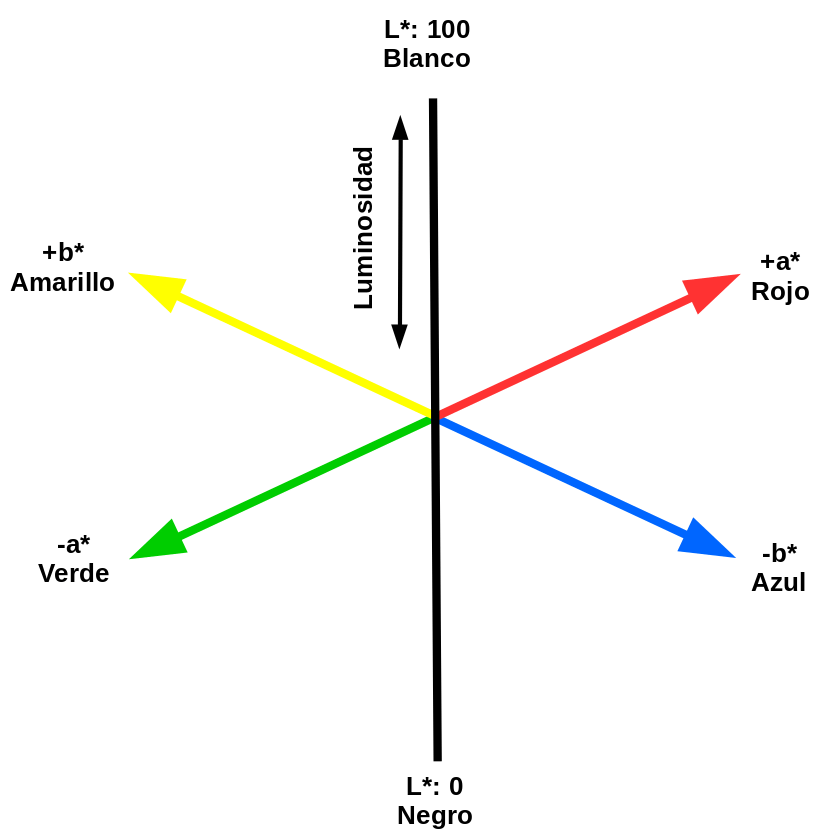
\includegraphics[width=0.38\linewidth]{figures/cie_lab.png}}
\end{figure}

\end{frame}
\begin{frame}{Análisis de color}
Se definen las máscaras $R_1, R_2, R_3, R_4$, para definir un espacio de color posible para el fuego, basado en los promedios de cada canal:


\[
R1(x,y) = 
\begin{cases}
    1, & \text{si } L^*(x,y) \geq L^*_m, \\
    0, & \text{caso contrario,}
\end{cases}
\]

\[
R2(x,y) = 
\begin{cases}
    1, & \text{si } a^*(x,y) \geq a^*_m, \\
    0, & \text{caso contrario,}
\end{cases}
\]

\[
R3(x,y) = 
\begin{cases}
    1, & \text{si } b^*(x,y) \geq b^*_m, \\
    0, & \text{caso contrario,}
\end{cases}
\]

\[
R4(x,y) = 
\begin{cases}
    1, & \text{si } b^*(x,y) \geq a^*(x,y), \\
    0, & \text{caso contrario,}
\end{cases}
\]

donde $L^*_m$, $a^*_m$, $b^*_m$ son los valores promedio de dicha componente en la imagen.
\end{frame}

\begin{frame}{Análisis de color}
Se define una última máscara $R_5$, de pixeles con mayor probabilidad de pertenecer a una región de fuego: 

\[
R5(x,y) = 
\begin{cases}
    1, & \text{si } P\big(L^*(x,y), a^*(x,y), b^*(x,y)\big) \geq \alpha, \\
    0, & \text{caso contrario,}
\end{cases}
\]

donde 
 \begin{itemize}
     \item $\alpha$ es un threshold
     \item $P\big(L^*(x,y), a^*(x,y), b^*(x,y)\big)$ es la probabilidad que $L^*$, $a^*$, $b^*$ pertenezcan a una región de fuego, calculada en base a un análisis con imágenes previamente segmentadas y etiquetadas.
 \end{itemize}    
\end{frame}

\begin{frame}{Detección de píxeles en movimiento}
\begin{itemize}
    \item Para determinar si un píxel $(x,y)$ está en movimiento en un tiempo $t$, generamos dos máscaras binarias para cada frame: \textbf{Foreground Difference} (FD), y \textbf{Background Difference} (BD).     
    \item Un píxel está \textbf{en movimiento} si $FD(x,y,t) = 1$ o $BD(x,y,t) = 1$
\end{itemize}
\end{frame}
\begin{frame}{Detección de píxeles en movimiento}
    \[
FD(x,y,t) = 
\begin{cases}
    1, & \text{si } \left| L^*(x,y,t) - L^*(x,y,t-1) \right| \geq T_{FD}, \\
    0, & \text{caso contrario,}
\end{cases}
\]

\[
BD(x,y,t) = 
\begin{cases}
    1, & \text{si } \left| L^*(x,y,t) - BG(x,y,t-1) \right| \geq T_{BD}, \\
    0, & \text{caso contrario,}
\end{cases}
\]
donde
\begin{itemize}
    \item $BG(x,y,t-1)$ es la luminosidad del fondo de la imagen en el instante $t-1$, obtenida analizando valores estáticos del frame previo. 

    \item $T_{FD}$ es la suma de la media $\mu$ y la desviación estándar $\sigma$ de $\left| L^*(x,y,t) - L^*(x,y,t-1) \right|$

    \item $T_{BD}$ es la suma de la media $\mu$ y la desviación estándar $\sigma$ de $\left| L^*(x,y,t) - BG(x,y,t-1) \right|$
        
\end{itemize}
\end{frame}

\begin{frame}{Análisis de regiones candidatas}
\begin{itemize}
    \item Se analizan las \textbf{componentes conexas} de los píxeles $(x,y)$ candidatos: aquellos segmentados tanto en el análisis de color como el de movimiento. 
    \item Se tienen en cuenta componentes conexas que \textbf{crecieron en área} en los últimos frames.
    \item \textbf{Idea}: en sus etapas tempranas, el fuego debe crecer espacialmente, por ende el número de píxeles detectados debería incrementar.
\end{itemize}
\end{frame}

\begin{frame}{Análisis de regiones candidatas}
    \begin{itemize}
        \item Llamamos $O(t)$ la componente conexa a analizar en el instante de tiempo $t$, y $NO(t)$ la cantidad de píxeles en $O(t)$.
        \item Definimos contador $CGO(t)$, que aumentará respecto al instante $t-1$ si en $t$ aumenta la cantidad de píxeles. Se actualiza como:
                \[
        CGO(t) =
        \begin{cases}
        CGO(t-1) + 1, & \text{si } NO(t) \geq NO(t-1) \\
        CGO(t-1), & \text{caso contrario.}
        \end{cases}
        \]
    \end{itemize}
\end{frame}

 \section{Evaluación}
\begin{frame}{Evaluación del método}
    Dados estos tres pasos, consideramos que el \textbf{algoritmo detectó fuego} si luego de aplicarlos a un frame, aún tenemos \textbf{píxeles de valor mayor a cero}.
\end{frame}
 
 \begin{frame}{Evaluación del método}
 Evaluamos la metodología presentada en dos instancias:
 \begin{itemize}
     \item Comparamos el resultado del análisis de color, con una segmentación realizada por el \textbf{algoritmo de Otsu sobre la componente $a^*$}.
     \item Para cada frame, comparamos estas tres opciones:
    \begin{itemize}
        \item El método original, es decir, $R_1, \dots, R_5$.
        \item Otsu sobre la componente $a^*$.
        \item Otsu sobre la componente $a^*$ combinado con $R_5$.
    \end{itemize}
 \end{itemize}
 \end{frame}
 
\begin{frame}{Algoritmo de Otsu}
\begin{itemize}
    \item Método para segmentar imágenes, propuesto por Nobuyuki Otsu$^2$
    \item En su versión más simple, separa la imagen en dos clases, y calcula un threshold que clasifica los píxeles en alguna de ellas.
    \item El threshold se calcula minimizando la varianza entre los píxeles de cada clase.
\end{itemize}
\end{frame}

\begin{frame}{Datos utilizados}
Utilizamos 4 videos (en total 763 frames)$^3$, buscando evaluar el método con videos de distintas características:
\begin{enumerate}
    \item Incendio en estación de servicio 
    \item Autopista sin fuego
    \item Incendio en bosque
    \item Incendio en patio, donde la iluminación de la escena es naranja
\end{enumerate}
 \end{frame}


\section{Resultados}
\begin{frame}{Experimento sobre método de segmentación}
Como primer experimento, realizamos solamente el paso de análisis de color sobre frames estáticos.
\end{frame}
\begin{frame}{Resultados}
    \begin{figure}
        \centering
        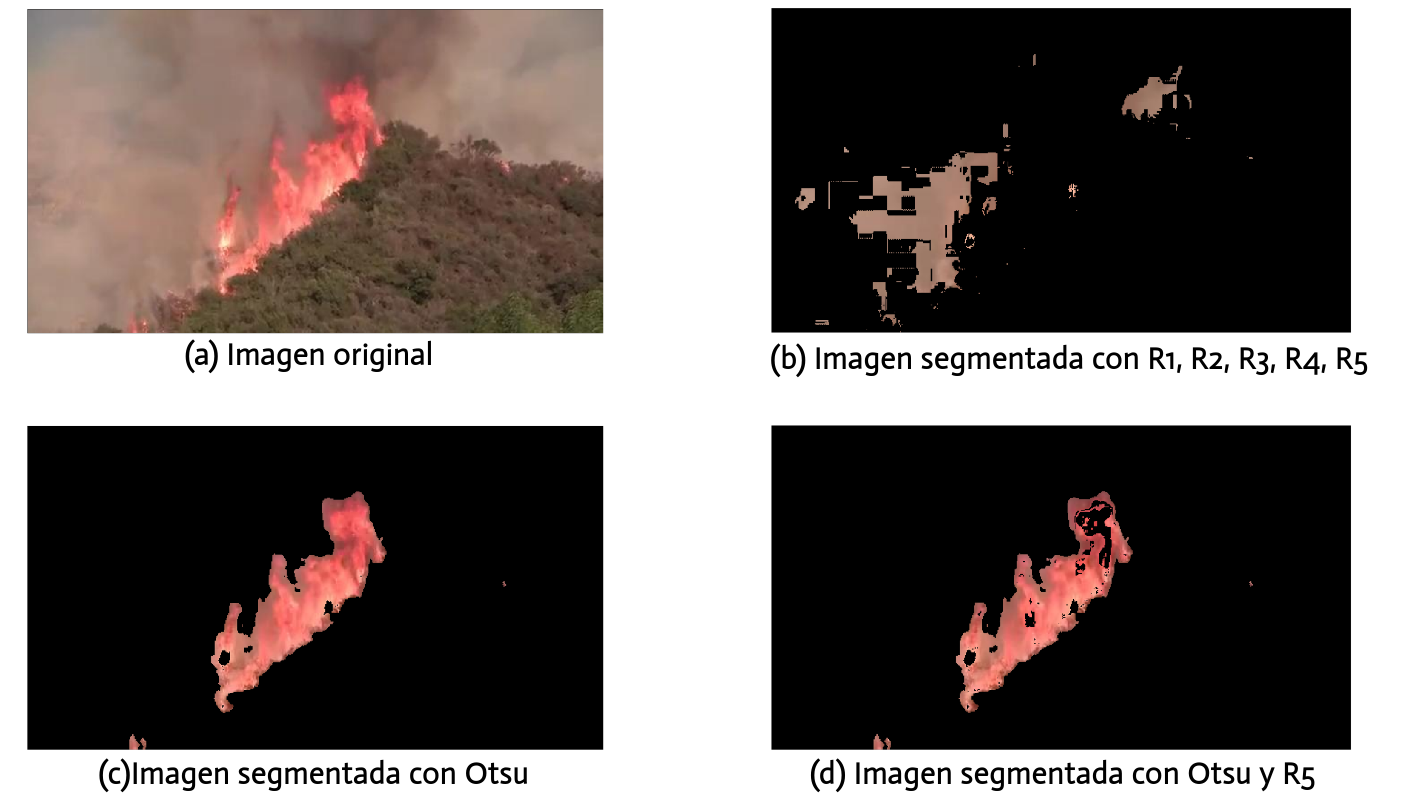
\includegraphics[width=1\linewidth]{figures/exp_img.png}
    \end{figure}
\end{frame}

\begin{frame}{Experimento sobre videos}
    A continuación, realizamos el método completo sobre los 4 videos mencionados.
    
    El video [1], de 69 frames, tuvo como resultados:
    \begin{figure}
        \centering
        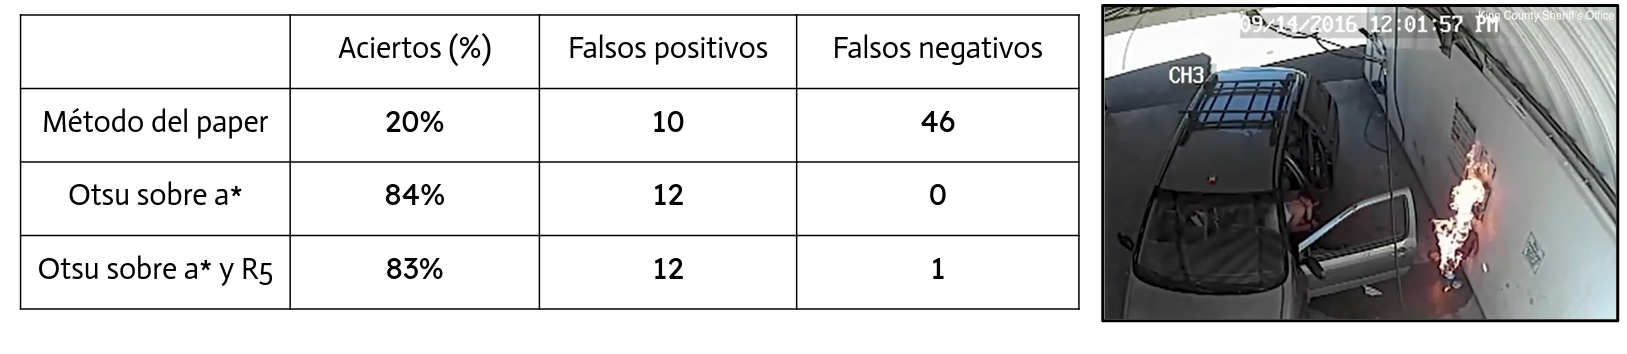
\includegraphics[width=1\linewidth]{figures/exp_video_1.png}
        \label{fig:exp_video_1}
    \end{figure}
\end{frame}

\begin{frame}{Experimento sobre videos}
    El video [2], de 26 frames, tuvo como resultados:
    \begin{figure}
        \centering
        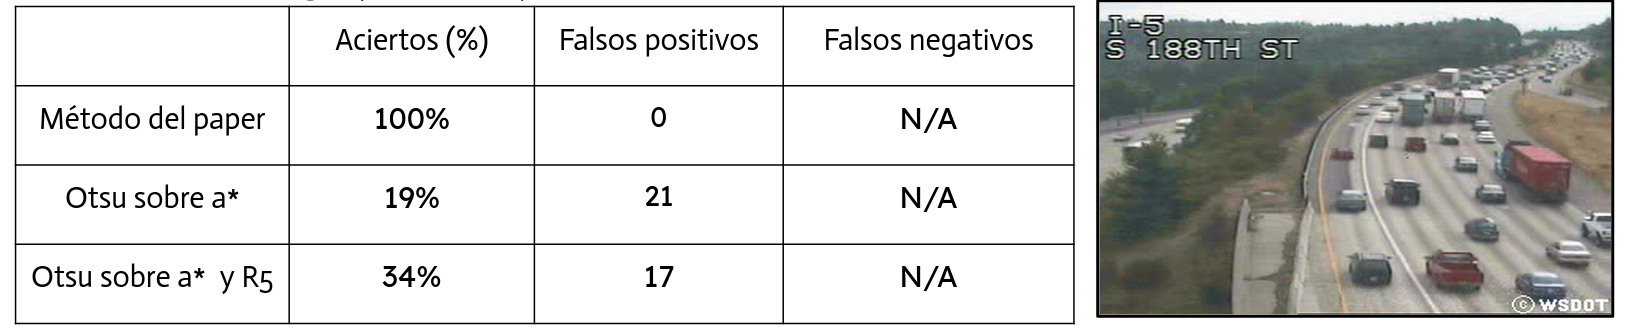
\includegraphics[width=1\linewidth]{figures/exp_video_2.png}
    \end{figure}
\end{frame}

\begin{frame}{Experimento sobre videos}
    El video [3], de 68 frames, tuvo como resultados:
    \begin{figure}
        \centering
        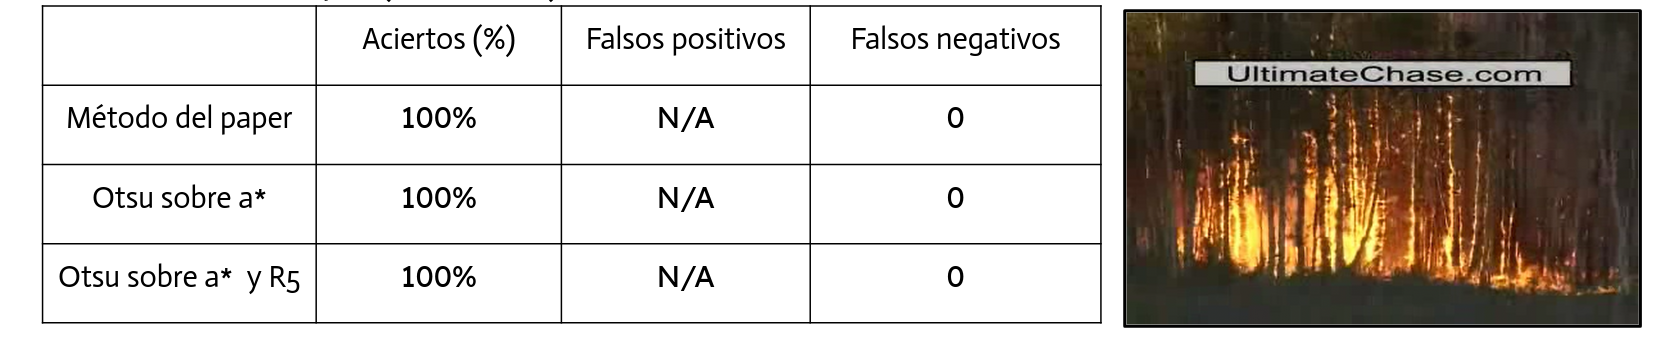
\includegraphics[width=1\linewidth]{figures/exp_video_3.png}
        \label{fig:exp_video_3}
    \end{figure}
\end{frame}

\begin{frame}{Experimento sobre videos}
    El video [4], de 600 frames, tuvo como resultados:

    \begin{figure}
        \centering
        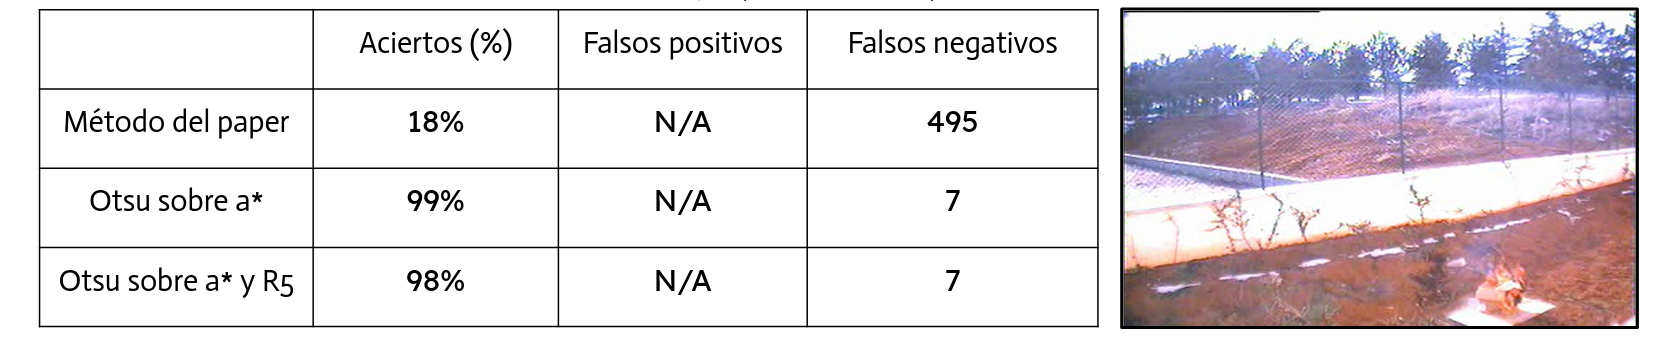
\includegraphics[width=1\linewidth]{figures/exp_video_4.png}
        \label{fig:exp_video_4}
    \end{figure}
\end{frame}


 \section{Conclusiones}
 \begin{frame}{Conclusiones}
    \begin{itemize}
        \item Para la tarea de \textbf{segmentación}, encontramos mejoras usando \textbf{Otsu} por sobre el método del paper. 
        \item Algunas suposiciones del método original no son siempre ciertas, en particular las relacionadas a su color que se usan para calcular $R_1,\dots,R_4$.
        \item El método original sigue teniendo mayor éxito
        \begin{itemize}
            \item  Sin embargo, notamos incidencia de \textbf{falsos negativos}, lo cual es poco deseable si el método se usa como refuerzo a una alarma de incendios.
        \end{itemize}
        
    \end{itemize}
 \end{frame}


\section{Referencias}
\begin{frame}{Referencias}
\bibliographystyle{abbrvnat}
\begin{thebibliography}{9}
\bibitem{paper} 
Celik, T. (2010).
\textit{Fast and efficient method for fire detection using image processing.} ETRI journal, 32(6), 881-890.

\bibitem{otsu} 
Otsu, N. (1975)
\textit{A threshold selection method from gray-level histograms}. Automatica, 11(285-296), 23-27. 

\bibitem{dataset} 
A. E. Çetin (2014) 
\textit{Computer Vision Based Fire Detection Dataset.}

\end{thebibliography}
\end{frame}

\end{document}